% !TEX root = ../main.tex

\chapter{控制系统仿真验证与分析}

\section{基于Simcenter STAR-CCM+的动力学参数求取}

水下机器人控制系统的模型精度直接影响姿态控制、深度控制和轨迹跟踪控制的仿真可信度。在第二章建立的六自由度动力学模型中，附加质量和水动力阻尼是影响ROV运动响应的重要水动力项。对于上述参数，工程上通常可通过CFD数值仿真或实机实验参数辨识两类方式获得。其中，实机辨识阻尼参数需要较准确的速度真值作为输入，而当前实验条件尚不具备水下动捕、多普勒测速仪等能够稳定提供ROV水下速度真值的测量设备。因此，本文采用基于CFD的平面运动机构（Planar Motion Mechanism, PMM）仿真方法，在Simcenter STAR-CCM+中对ROV进行水动力参数求取，并将结果用于后续MATLAB/Simulink控制系统仿真。

\subsection{流体域建立与网格划分}

在导入STAR-CCM+之前，首先在Fusion中对机器人三维模型进行网格前处理。由于ROV本体由框架、推进器安装座、浮力材料、耐压舱和传感器舱等部件组成，局部存在小圆角、薄壁边缘、安装孔和相邻零件间的窄缝。若直接将原始CAD模型导入CFD软件，复杂曲面在自动表面重构过程中容易出现局部面片过粗、边界识别不连续或细小特征丢失等问题，进而影响布尔扣除、棱柱层生成和后续流体力积分结果。因此，本文在Fusion中先对模型进行必要的简化和细分网格处理：删除与外部绕流影响较小的内部螺纹、倒角和装配细节，保留会显著改变迎流面积和尾流结构的框架、舱体及推进器外形；随后提高曲面离散精度，对圆柱舱体、推进器导管和框架交界区域进行局部细分，使导出的表面网格能够更准确描述机器人外形。

经过Fusion前处理后，模型表面三角面片分布更加均匀，尖锐边界和曲率变化区域得到更稳定的表达。一方面，这可以减少STAR-CCM+自动表面修复时产生的非物理封补和破面；另一方面，也有助于后续体网格在复杂几何附近形成平滑过渡，降低负体积网格和网格畸变出现的概率，从而提高非定常PMM仿真的收敛稳定性和水动力参数求取精度。

\begin{figure}[htbp]
    \centering
    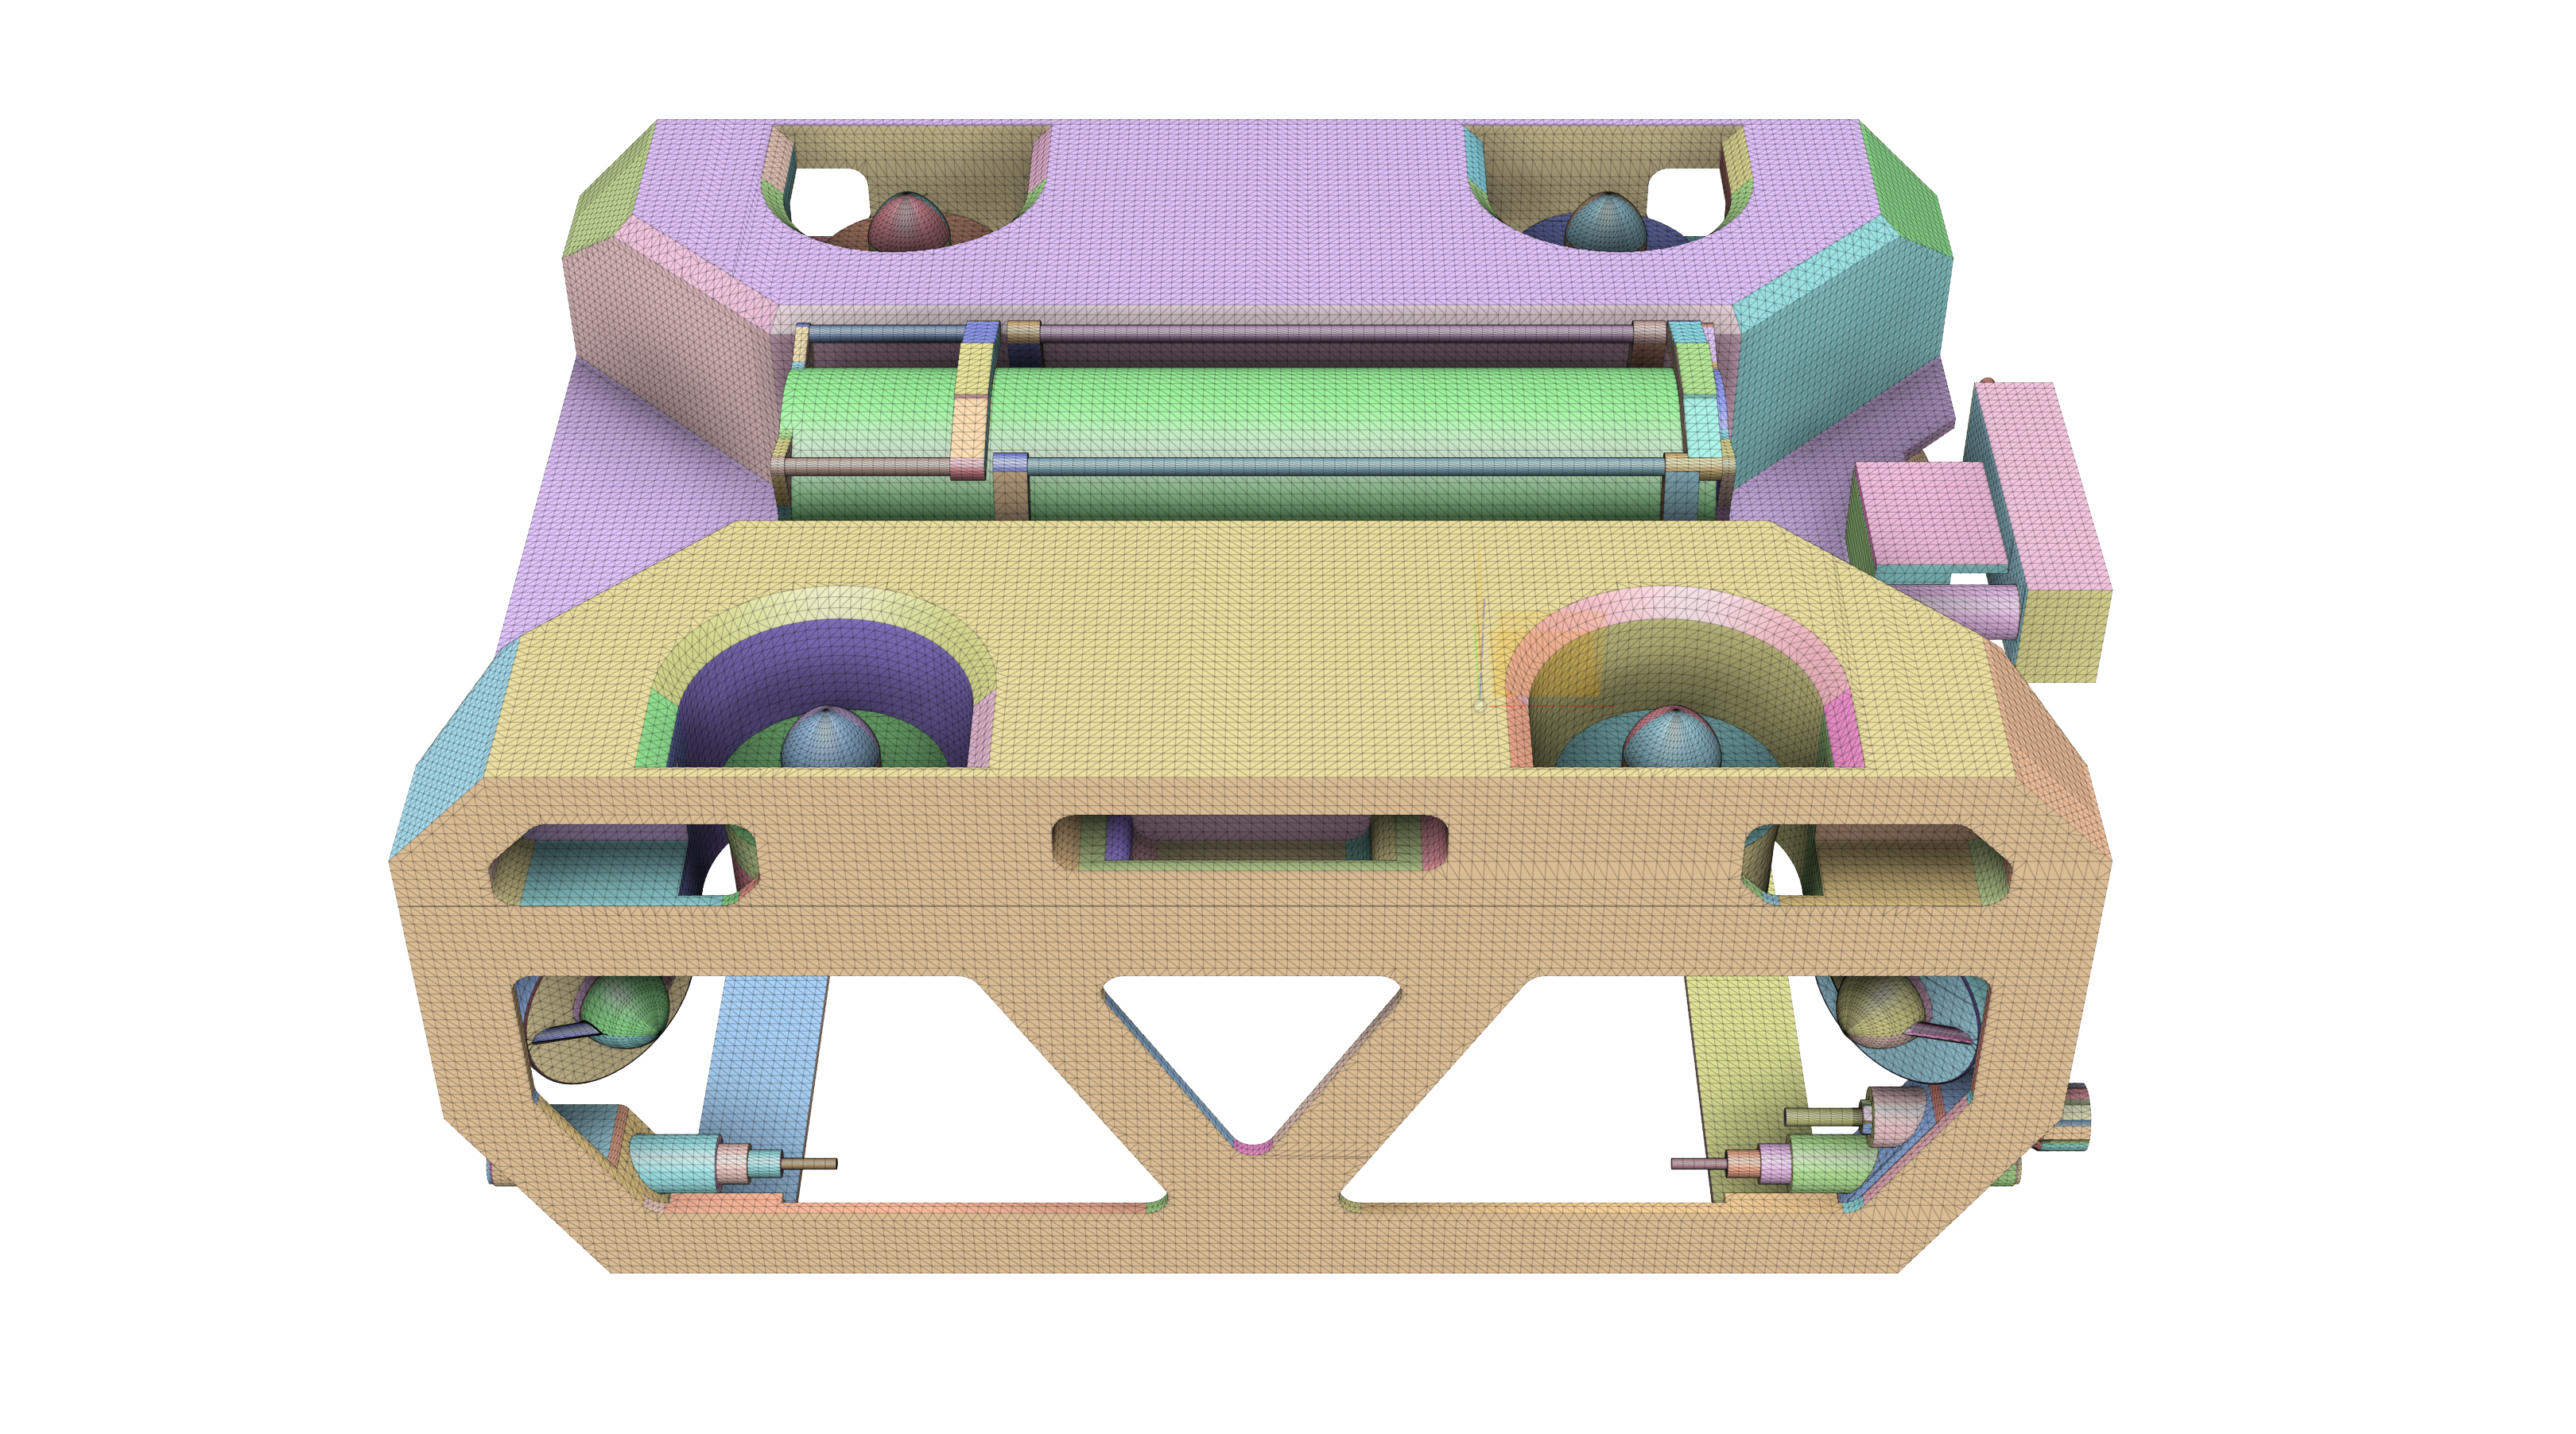
\includegraphics[width=0.82\textwidth]{../figures/CFD-PRE.png}
    \caption{Fusion中CFD前处理与表面网格细分效果}
    \label{fig:cfd_preprocess_fusion}
\end{figure}

完成模型前处理后，将机器人模型导入Simcenter STAR-CCM+中建立虚拟拖曳水池。计算域采用长方体流体域，并通过布尔差运算从流体域中扣除机器人实体区域，从而得到真实的外部流体计算区域。为减小边界对机器人绕流结果的影响，流体域在机器人前方、后方、侧向和垂向均保留足够距离。入口边界用于给定来流速度，出口边界采用压力出口，其余外边界采用对称或滑移边界处理，机器人表面设置为无滑移壁面。

网格划分采用自动网格流程，主要包括表面重构、自动表面修复、多面体体网格以及棱柱层网格。表面重构用于提高复杂曲面区域的网格一致性；自动表面修复用于处理导入模型中可能存在的微小缝隙和非匹配边；多面体网格在复杂外形附近具有较好的稳定性和收敛性；棱柱层网格用于刻画机器人表面附近的速度梯度和边界层效应。本文采用的主要网格参数如表~\ref{tab:starccm_mesh_parameters}所示。

\begin{table}[htbp]
    \centering
    \caption{STAR-CCM+网格划分主要参数设置}
    \label{tab:starccm_mesh_parameters}
    \begin{tabular}{cc}
        \hline
        参数 & 设置值 \\
        \hline
        基础尺寸 & $0.01\,\mathrm{m}$ \\
        目标表面尺寸 & $100\%$，即 $0.01\,\mathrm{m}$ \\
        最小表面尺寸 & $0.675\%$，即 $6.75\times10^{-5}\,\mathrm{m}$ \\
        表面曲率 & 36 \\
        表面网格增长率 & 1.3 \\
        自动修复最小接近值 & 0.001 \\
        棱柱层数 & 10 \\
        棱柱层总厚度 & $0.008\,\mathrm{m}$ \\
        最大网格单元尺寸 & $0.04\,\mathrm{m}$ \\
        \hline
    \end{tabular}
\end{table}

图~\ref{fig:starccm_body_and_domain_mesh}展示了机器人本体附近的局部网格和整个流体域的网格划分结果。可以看出，在机器人外形和棱边附近网格被自动加密，而远离机器人本体的流体域采用较大的网格尺寸，从而在保证流体力计算精度的同时控制了整体计算量。

\begin{figure}[htbp]
    \centering
    \begin{minipage}[t]{0.48\textwidth}
        \centering
        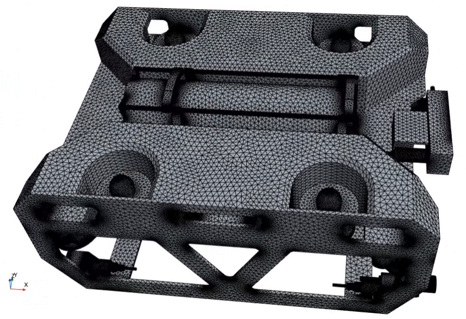
\includegraphics[width=\textwidth]{../figures/starccm_body_mesh.png}
        \\(a) 水下机器人本体附近网格划分
    \end{minipage}
    \hfill
    \begin{minipage}[t]{0.48\textwidth}
        \centering
        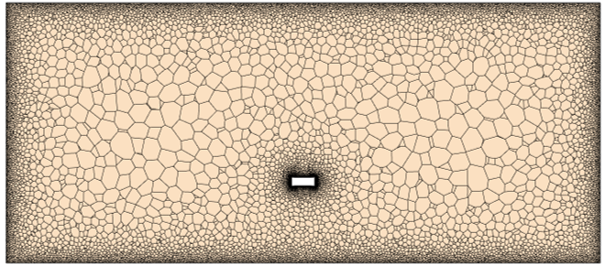
\includegraphics[width=\textwidth]{../figures/starccm_domain_mesh.png}
        \\(b) 整个流体域网格划分
    \end{minipage}
    \caption{STAR-CCM+中水下机器人本体与流体域网格划分结果}
    \label{fig:starccm_body_and_domain_mesh}
\end{figure}

\subsection{仿真工况设置}

仿真物理模型采用三维不可压水介质，密度设置为常数，湍流模型选用$k$-$\omega$类RANS模型，以兼顾机器人绕流分离、尾流结构捕捉和计算效率。求解器采用非定常求解方式，通过平面运动机构（Planar Motion Mechanism, PMM）思想设置单自由度强迫运动工况，分别获得机器人在纵荡、横荡、垂荡、横摇、纵摇和艏摇方向上的流体力与流体力矩响应。

PMM仿真区域由外部静止域和内部运动域组成。外部计算域尺寸设置为$10\,\mathrm{m}\times8\,\mathrm{m}\times5\,\mathrm{m}$，内部运动域采用直径$1.2\,\mathrm{m}$、长度$1.6\,\mathrm{m}$的圆柱区域包络机器人本体。该设置能够在保证机器人周围非定常流场解析精度的同时，使运动区域与远场边界保持足够距离，从而减小边界反射和网格变形对流体力计算结果的影响。对于运动域与外部静止域之间的交界面，采用滑移网格或重叠网格方式传递流场信息，以满足强迫运动过程中网格质量和求解稳定性的要求。

在各方向PMM工况中，STAR-CCM+记录机器人壁面压力力、黏性力及对应力矩的时间历程。本文将所得结果直接用于后续动力学模型中的水动力参数设定，忽略数值较小的非对角耦合项，仅保留六自由度方向上的主要对角项，以降低控制仿真模型复杂度并满足嵌入式控制器实时计算需求。

图~\ref{fig:starccm_velocity_contour}给出了典型工况下机器人周围速度云图。从速度分布可以看出，机器人框架和推进器安装区域附近存在明显的局部加速与尾流结构，这也是水下机器人阻尼参数具有显著非线性的主要原因之一。

\begin{figure}[htbp]
    \centering
    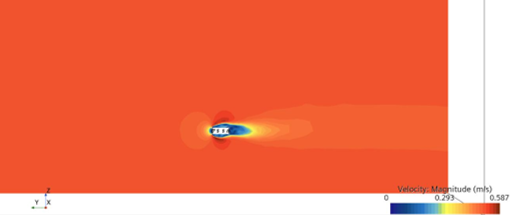
\includegraphics[width=0.82\textwidth]{../figures/starccm_velocity_contour.png}
    \caption{典型工况下水下机器人周围速度云图}
    \label{fig:starccm_velocity_contour}
\end{figure}

\subsection{水动力参数结果}

基于上述CFD仿真结果，本文忽略数值较小的非对角耦合项后，得到的六自由度附加质量矩阵为
\begin{equation}
    \boldsymbol{M}_{A}=
    \operatorname{diag}\left(
    3.7716,\ 12.7006,\ 16.4712,\ 0.0545,\ 1.2628,\ 0.8198
    \right),
    \label{eq:added_mass_matrix_chap5}
\end{equation}
线性阻尼矩阵为
\begin{equation}
    \boldsymbol{D}_{L}(\boldsymbol{\nu})=
    \operatorname{diag}\left(
    5.9341,\ 4.3172,\ 6.2491,\ 0.0199,\ 0.4611,\ 0.0698
    \right),
    \label{eq:linear_damping_matrix_chap5}
\end{equation}
二次阻尼矩阵为
\begin{equation}
    \boldsymbol{D}_{Q}(\boldsymbol{\nu})=
    \operatorname{diag}\left(
    19.374,\ 42.687,\ 51.0402,\ 0.0668,\ 1.9172,\ 1.1343
    \right).
    \label{eq:quadratic_damping_matrix_chap5}
\end{equation}
其中，前三个元素对应纵荡、横荡和垂荡方向，后三个元素对应横摇、纵摇和艏摇方向。由结果可知，垂荡方向附加质量和阻尼参数均相对较大，说明机器人在垂直方向运动时需要带动更多周围流体并受到较明显的流体阻力影响；横荡方向的二次阻尼明显大于纵荡方向，表明机器人侧向投影面积和框架结构对横向运动阻力具有较强影响。旋转自由度中，纵摇方向的附加转动惯量和阻尼参数高于横摇、艏摇方向，说明机器人在纵向俯仰运动时更容易受到浮体、框架和推进器安装结构带来的水动力矩影响。

上述参数将作为后续控制系统仿真模型中的附加惯性项和水动力阻尼项，并与刚体惯性参数、浮力重力项和推进器分配模型共同构成水下机器人六自由度动力学模型。通过在仿真模型中引入STAR-CCM+得到的$\boldsymbol{M}_{A}$、$\boldsymbol{D}_{L}(\boldsymbol{\nu})$和$\boldsymbol{D}_{Q}(\boldsymbol{\nu})$，可以提高控制算法仿真结果与实际水动力响应之间的一致性。

\section{推进器推力拟合}

在第三章的推力分配算法中，控制器输出首先被解算为各推进器所需提供的期望推力。若要在实机系统中准确执行该推力指令，还需要进一步建立推进器推力与电调油门之间的映射关系。推进器推力拟合的目的即是为模型控制中的精确推力控制服务，使控制系统能够将期望推力准确转换为对应油门值，从而实现对每个推进器的独立、可重复推力控制。

由于水下推进器的输出推力受到螺旋桨、电机、电调、电源电压以及安装方式等因素影响，单纯依靠厂家标称曲线难以完全反映本文实验系统中的实际输出特性。尤其在电池供电条件下，母线电压会随放电过程发生变化，同一油门指令在不同电压下可能对应不同的实际推力。因此，本文搭建实机推力测试台架，测试不同供电电压和不同油门指令下的稳定推力，并根据实验数据建立推进器推力反查表。该反查表随后用于控制程序中的期望推力到油门反解，使仿真模型中的推进器推力指令能够与实机执行层保持一致。

\subsection{推力测试台架搭建}

推力测试系统主要由水下推进器、一维力传感器、数据采集器、STM32F4开发板、电调及可调直流电源组成。考虑到测试需要在水下环境中长时间进行，力传感器选用能够在水下稳定工作的单轴力传感器，用于测量推进器轴向推力。测试台架采用铝型材框架搭建，以保证整体结构刚度和装配调整便利性；推进器固定在框架一端，力传感器布置在推进器推力方向上，使推进器产生的轴向载荷能够直接传递至传感器测量端。

力传感器输出信号接入数据采集器，由数据采集器完成信号调理和数字化转换。STM32F4开发板通过MODBUS-RTU协议向数据采集器发送数据请求，周期性读取当前推力测量值；同时，开发板通过DSHOT协议向电调发送油门指令，控制推进器在不同油门下运行。该测试链路与第四章所述底层通信框架保持一致，能够在实际嵌入式控制器上完成油门下发、推力采样和实验数据记录。

实验过程中，在推进器工作电压范围内选取多组供电电压，并在每个电压点下依次给定多组正、反向油门指令。每个电压--油门组合保持一段稳定运行时间，待传感器读数进入稳定区间后记录平均推力值，从而得到离散的电压--油门--推力数据表。为降低瞬态启动、螺旋桨尾流波动和传感器噪声对结果的影响，本文对每个测试点采集多次数据，并取稳定段均值作为该电压和油门组合下的标定推力。

\subsection{推力曲线拟合方法}

实机控制中需要解决的是期望推力到油门的反解问题，即在已知当前供电电压$U$和期望推力$T_d$的条件下，求得应下发至电调的油门指令$\delta_d$。由于推进器推力不仅与油门有关，还会受到供电电压影响，本文将标定得到的电压--油门--推力离散数据整理为二维反查表，并建立如下映射：
\begin{equation}
    \delta_d=g(T_d,U),
    \label{eq:thruster_force_fit}
\end{equation}
其中$g(\cdot)$表示由实验标定数据构成的二维插值关系。对于正向推力和反向推力区间，分别建立对应的反查表，以适应推进器正反转效率不完全一致的情况。

在线控制时，控制器首先根据推力分配结果得到单个推进器的期望推力$T_d$，同时读取当前母线电压$U$；随后在二维反查表中查找相邻网格点，并通过双线性插值计算目标油门$\delta_d$。本文在STM32F4嵌入式平台上采用ARM CMSIS-DSP库中的\texttt{arm\_bilinear\_interp\_f32}函数实现该过程。该函数针对ARM Cortex-M系列处理器的浮点运算单元进行了底层优化，能够减少在线插值计算开销，适合部署在需要高频更新油门指令的嵌入式控制系统中，从而保证推力反解的实时性。

\subsection{推力控制准确性验证}

为验证推力拟合结果在实机控制中的有效性，本文进一步进行期望推力跟踪测试。实验时，首先给定一组期望推力序列$T_d$，控制程序结合当前供电电压$U$，根据已建立的二维反查表通过双线性插值计算得到对应油门$\delta_d$，并通过DSHOT协议更新至电调。推进器达到稳定状态后，由一维力传感器测得实际推力$T_m$，并将其与期望推力进行对比。

对于$n$组测试数据，推力控制误差可表示为
\begin{equation}
    e_i=T_{m,i}-T_{d,i},\quad i=1,2,\dots,n,
\end{equation}
并采用均方根误差评价整体控制精度：
\begin{equation}
    \operatorname{RMSE}=
    \sqrt{\frac{1}{n}\sum_{i=1}^{n}\left(T_{m,i}-T_{d,i}\right)^2}.
    \label{eq:thruster_rmse}
\end{equation}
通过多组期望推力测试可以看出，插值反解得到的油门指令能够较准确地驱动推进器输出目标推力，传感器测得推力与期望推力之间误差较小，说明本文建立的推进器推力拟合关系能够满足ROV模型控制中精确推力执行的需求。

\section{基于MATLAB/Simulink的仿真环境搭建}

\subsection{实机实验}

\section{本章小结}
